\documentclass[lettersize,journal]{IEEEtran}
\usepackage{amsmath,amsfonts}
\usepackage{algorithmic}
\usepackage{array}
\usepackage[caption=false,font=normalsize,labelfont=sf,textfont=sf]{subfig}
\usepackage{textcomp}
\usepackage{stfloats}
\usepackage{url}
\usepackage{verbatim}
\usepackage{graphicx}
\usepackage{booktabs}
\usepackage{multirow}  
\hyphenation{op-tical net-works semi-conduc-tor IEEE-Xplore}
\def\BibTeX{{\rm B\kern-.05em{\sc i\kern-.025em b}\kern-.08em
    T\kern-.1667em\lower.7ex\hbox{E}\kern-.125emX}}
\usepackage{balance}
% 设置超链接跳转
\usepackage[colorlinks,
linkcolor=blue,
anchorcolor=blue,
citecolor=blue]{hyperref} 
\usepackage{amsmath}

% 改变字体颜色
\usepackage{color,xcolor}
\usepackage{makecell}
\begin{document}
\title{UVDT: Digital Twin of Urban Vehicles Based on LiDAR-Camera Fusion in Multi-Intersection Scenarios}
\author{IEEE Publication Technology Department

\thanks{Manuscript created October, 2020; This work was developed by the IEEE Publication Technology Department. This work is distributed under the \LaTeX \ Project Public License (LPPL) ( http://www.latex-project.org/ ) version 1.3. A copy of the LPPL, version 1.3, is included in the base \LaTeX \ documentation of all distributions of \LaTeX \ released 2003/12/01 or later. The opinions expressed here are entirely that of the author. No warranty is expressed or implied. User assumes all risk.}}

\markboth{Journal of \LaTeX\ Class Files,~Vol.~18, No.~9, September~2020}%
{How to Use the IEEEtran \LaTeX \ Templates}

\maketitle

\begin{abstract}
In this paper, we explore the application of digital twins in automated driving and propose Urban Vehicle Digital Twin(UVDT), which replicates the traffic flow by investigating four aspects: single-intersection multi-object tracking, multi-intersection multi-object tracking, trajectory inference and reduction, and twinning. 
The multi-object tracking performance is optimized by fusing radar detection and camera detection data to improve the accuracy and robustness of vehicle detection, which in turn solves the challenges posed by occlusion and view angle changes. 
Cross-scene vehicle re-recognition is improved by generating rich training data. 
The digital twin-based vehicle control method provides high-precision path planning and control for the autonomous driving system, ensuring accurate vehicle navigation in complex traffic scenarios. 
The experimental results show that UVDT can provide high-fidelity simulation scenarios for the testing and optimization of autonomous driving systems, which promotes the development of intelligent transportation systems and provides important support for the construction of future smart cities.
\end{abstract}

\begin{IEEEkeywords}
digital twins, automated driving, vehicle detection, multi-object tracking, trajectory reduction.
\end{IEEEkeywords}


\section{Introduction}

\IEEEPARstart{W}{ith} the rapid development of intelligent transportation, autonomous driving, and urban management, digital twin technology, as an important innovative tool, has gradually shown tremendous potential in various fields\cite{Alpher17}. 
A digital twin refers to the creation of a digital model corresponding to the real world through the real-time synchronization of data collected from the physical world and virtual models\cite{Alpher20c}. 
This technology can simulate, analyze, and optimize the real world in a virtual environment, thus providing support for decision-making\cite{Alpher21b}. 
In the field of autonomous driving, digital twin technology can accurately replicate factors such as traffic flow, road structure, and pedestrian behavior, providing a precise testing and training environment for the perception, planning, and control of autonomous driving systems\cite{Alpher24}\cite{Alpher20d}.

The focus of this research is to apply digital twin technology to the development and testing of autonomous driving systems to improve the interpretability and robustness of autonomous driving systems by replicating real traffic flow scenarios\cite{Alpher24b}.
By constructing high-precision digital twin models and combining reinforcement learning with simulation platforms, we are able to simulate complex driving scenarios and train and optimize autonomous driving algorithms\cite{Alpher22c}. 
At the same time, digital twin technology can provide smarter decision support for traffic management, promoting the development of smart city construction\cite{Alpher17b}.

\begin{figure}[t]
	\centering
	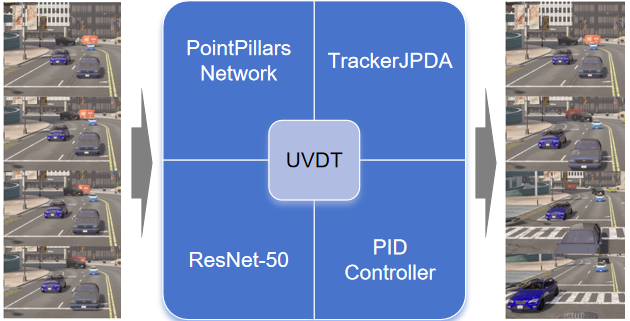
\includegraphics[width=\linewidth]{picture/picture1.png} 
	\caption{Overall Preview of Digital Twin through UVDT} 
	\label{fig:example} 
\end{figure}

We primarily conducted research from four aspects: single-intersection multi-target tracking, multi-intersection multi-target tracking, trajectory inference and restoration, and digital twinning. 
By fusing camera and radar detection, we improved the accuracy of vehicle detection, addressing challenges such as occlusion and perspective changes, thereby optimizing multi-target tracking performance. 
We collected a large amount of training data to train the tracking model, further enhancing tracking performance. 
We inferred trajectories in unknown regions and combined them with the trajectories obtained from multi-target tracking within intersections, ultimately achieving complete trajectories. 
Using the PID control algorithm, we implemented digital twinning by following the previously obtained trajectories.

Vehicle detection is a core perception task in autonomous driving systems, which usually relies on data from various sensors (such as lidar, cameras, and millimeter-wave radar) for object recognition and positioning. As a key input source for digital twin systems, the accuracy of vehicle detection directly affects the behavior modeling and scene restoration quality of traffic participants in virtual environments. 
In recent years, the application of deep learning technologies has significantly improved the accuracy and robustness of vehicle detection. 
On the contrary, through digital twin technology, we can create precise virtual environments to provide abundant training data for autonomous driving systems, enhancing detection performance. 
Digital twins not only improve detection effectiveness in complex and dynamic environments but also optimize the fusion of data from different sensors\cite{Alpher20}.

Object tracking is a key technology in autonomous driving, particularly in multi-object tracking, where the task becomes especially complex due to target occlusions, changes in viewpoint, and misalignment between multiple cameras. 
The accuracy and robustness of object tracking directly affect the credibility of the digital twin system, and its output results (such as target ID consistency and trajectory continuity) can be used to verify the timing consistency of sensor simulation in the virtual environment, detect physical rule deviations in scene modeling, and optimize the motion prediction algorithm of the digital twin.
When the tracking algorithm has ID switching or trajectory breakage in complex scenes, these abnormal data can reveal the potential defects of the digital twin system in terms of dynamic object interaction, multi-sensor synchronization, or environment rendering accuracy, thereby providing data support for the iterative optimization of the simulation model and continuously enhancing the environmental authenticity and behavioral reliability of the digital twin system\cite{Alpher22b}.

Vehicle re-identification (Re-ID) refers to recognizing the same vehicle at different times and locations, especially across multiple viewpoints and different cameras. 
By constructing a vehicle dataset with continuous time series, variable perspectives and dynamically changing environments in a virtual simulation environment, rich feature learning materials are provided for the training of the re-identification algorithm.
The trained algorithm can not only effectively distinguish the skeleton models of different vehicles through precise feature matching, but also accurately identify the color changes of the same vehicle under different lighting conditions, thereby providing a reliable identity association basis for vehicle tracking in multi-camera scenarios, and ensuring the continuity and consistency of vehicle motion trajectories in complex environments\cite{Alpher23}.
This technical path based on virtual data training and real scene verification not only improves the robustness of the re-identification algorithm, but also lays a solid foundation for the precise tracking of intelligent transportation systems.

Trajectory restoration aims to reconstruct complete and continuous vehicle motion trajectories in complex urban road environments through advanced algorithms.
In practical applications, due to the detection distance limitations of multi-target trackers, coupled with interference factors such as target occlusion and sensor noise, tracking interruptions and trajectory breaks often occur.
To meet this challenge, the system needs to combine kinematic models and deep learning algorithms to intelligently infer and complete the lost trajectory fragments to ensure the spatiotemporal continuity of the trajectory.
Finally, by accurately simulating the vehicle's driving route and traffic behavior through integrated control algorithms, a complete autonomous driving system verification platform is formed, providing a reliable digital twin foundation for algorithm development and safety assessment\cite{Alpher24c}.

\section{Related Work}

We have summarized research work on different aspects of UVDT.

\textbf{Vehicle Detection.}
UVDT mainly uses LiDAR and cameras for vehicle object detection.
Several recent studies have explored the fusion of LiDAR and camera data for vehicle detection,demonstrating significant improvements in both accuracy and robustness. 
For instance, MVDNet (2018) utilizes a multi-view fusion approach, where LiDAR point clouds are projected to different views (such as bird’s-eye view and front view) and matched with camera images, combining depth information from LiDAR and texture information from the camera. 
This method improves detection performance, especially in complex environments\cite{Alpher22h}. 
Building on this, PointPillars introduces a fast encoder for LiDAR data, using a grid-based encoding approach that could potentially be integrated with camera data in future fusion methods to enhance detection speed and efficiency\cite{Alpher19}.
Another study combines LiDAR and camera data by feeding them into separate convolutional neural networks, where the features extracted from both modalities are fused to perform object detection\cite{Alpher20e}. 
This approach has shown significant improvements in detection performance, particularly in dynamic environments with occlusions or sparse LiDAR data.
Lastly, ST-MVDNet introduces a self-training framework using a teacher-student mutual learning mechanism, where the teacher network is trained on the fused LiDAR and camera data, while the student network is exposed to strong data augmentation simulating missing sensor modalities\cite{Alpher22f}. 

This approach enhances the model’s robustness against sensor failures by ensuring consistency between the teacher and student models, allowing the system to better handle missing or noisy data during inference.
These methods collectively highlight the importance of sensor fusion and advanced learning techniques in achieving robust and accurate vehicle detection, even in challenging conditions.
We use a combination of PointPillars-based 3D point cloud detection method and YOLOv4-based 2D image detection method for multimodal object detection.
These two deep learning methods have shown excellent detection performance in their respective fields.

\textbf{Multi-Object Tracking.}
Specker and his team proposed an online multi-camera multi-target tracking method (OCMCTrack), which dynamically optimizes cross-camera target association through an innovative Corrective Matching Cascade strategy, significantly improving tracking accuracy and ID consistency in complex scenarios while ensuring real-time processing\cite{Alpher24e}.
Shim and his team proposes a robust multi-target multi-camera vehicle tracking system designed for city-scale traffic management, addressing challenges like occlusion and cross-camera identity consistency by integrating spatial-temporal constraints and deep feature fusion to enable real-time vehicle monitoring and behavior analysis across urban camera networks\cite{Alpher21e}.
Most existing algorithms, with a few exceptions, can be seen as special cases of the multi-modal fusion problem. 
These methods organize the input data using a graph structure, where edges represent relationships between modalities, and nodes represent different targets or states. 
Algorithms that can be solved in polynomial time typically handle specific modalities or time-continuous edges, with some also utilizing maximum flow or matching algorithms. 
Methods that leverage global information (beyond just time continuity or modality constraints) can significantly improve performance, but they are usually NP-hard due to the involvement of combinatorial optimization. 
In some cases, marginal terms or local constraints are added to ensure completeness. 
To enhance model expressiveness, some studies have employed higher-order relations, although the gains diminish significantly as complexity increases. 
Joint optimization and iterative optimization strategies have also been widely used to improve performance.
We use Joint Integrated Probabilistic Data Association (JIPDA), which combines data from multiple sensors and optimizes probabilistic associations to effectively handle data uncertainty and missing information in target tracking, improving tracking accuracy and robustness in complex environments.


\textbf{Vehicle Reidentification.}
Bing and his team proposed a part-based regularization method, which enhances the accuracy of vehicle re-identification by detecting local parts of vehicles, such as lights and wheels\cite{Alpher19b}. 
Zheng and his colleagues introduced a large-scale vehicle re-identification dataset named VehicleNet and proposed a multi-task learning framework that combines vehicle re-identification and vehicle attribute recognition tasks, improving the model's generalization capability\cite{Alpher20f}. 
P and the research team proposed a dual-path model that integrates global and local features and incorporates an adaptive attention mechanism to enhance the accuracy of vehicle re-identification\cite{Alpher19c}.

The most advanced technologies in the field of vehicle re-identification currently include the combination of deep convolutional neural networks (CNN) for feature extraction and metric learning\cite{Alpher20g}, particularly with the integration of cross-view and cross-domain learning techniques, the use of Generative Adversarial Networks (GAN) for image enhancement\cite{Alpher21d}, and the fusion of multi-sensor data (such as cameras, radar, and LiDAR) to improve the model's robustness and accuracy in complex environments\cite{Alpher22g}.

Inspired by person Re-ID techniques for video sequences, we developed a retrained vehicle Re-ID network based on ResNet-50. 
The network has acquired comprehensive feature representations through large-scale image training, enabling effective vehicle re-identification performance.

\begin{figure*}[t]
	\centering
	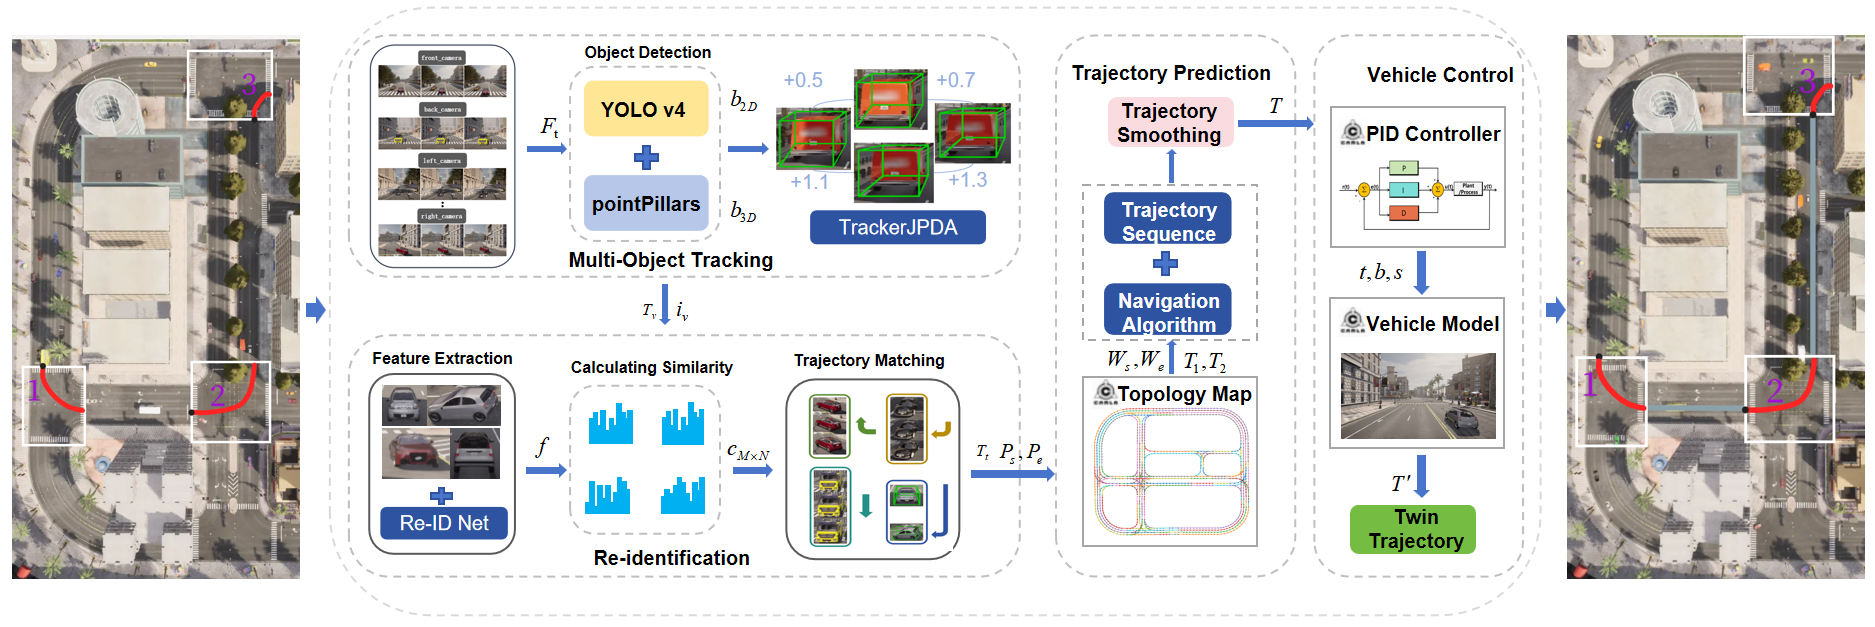
\includegraphics[width=\textwidth]{picture/picture2.png} 
	\caption{Given the original scene, cameras and radar detect vehicles, and the tracker performs single-camera multi-target tracking and multi-camera multi-target tracking. The data obtained from tracking is used for trajectory reconstruction, and finally, a digital twin is created to replicate the traffic scenario.}
	\label{fig:example}
\end{figure*}

\textbf{Digital Twin.}
After obtaining the trajectory data of all tracked vehicles, we will use the vehicle control algorithm to reproduce the traffic flow in the simulation scenario.
Kaleb Ben Naveed et al. proposed a hierarchical reinforcement learning-based method for autonomous driving trajectory planning and control. 
By training a reinforcement learning agent in a simulation environment, this method optimizes the vehicle's control strategy according to environmental changes, achieving efficient trajectory planning and dynamic path adjustment.\cite{Alpher22}
R. Barea et al. proposed a deep reinforcement learning (DRL)-based control method, where an agent is trained in the CARLA simulation platform to autonomously learn and optimize the vehicle's control strategies (such as throttle, brake, and steering) to ensure safe and smooth driving.\cite{Alpher21}
We optimize the trajectories obtained from multi-object tracking using a trajectory smoothing algorithm, enabling the vehicle to turn more smoothly and drive more steadily (reducing bumps and sudden maneuvers) while ensuring precise adherence to the planned path at a lower computational cost. 
Subsequently, the PID controller is employed to control the vehicle, guiding it to follow the optimized trajectory and achieve final trajectory-tracking synchronization.


\section{Method}

\subsection{Problem Definition}

In UVDT, the vehicle detection and tracking system for single-intersection scenarios adopts a multimodal data fusion architecture.
The input source integrates 3D point cloud data captured by LiDAR and synchronized RGB images from six calibrated cameras, achieving heterogeneous sensor data collaboration through spatiotemporal alignment.
The input for multi-intersection object detection is the same as that for a single intersection, but the input for its object tracking includes trajectories and the corresponding vehicle appearance features. 
The input for the re-identification module is a N×2048 vehicle feature vector. 
The input for the twin part includes trajectory data (comprising the desired vehicle trajectory and the current vehicle state), environmental information (such as road conditions and obstacle information), and the system's control strategy.

\textbf{PointPillars.}
We use the PointPillars network to process the input for vehicle detection and generate the output.
A PointPillars network requires two inputs: pillar indices as a P-by-2 and pillar features as a P-by-N-by-K matrix. P is the number of pillars in the network, N is the number of points per pillar, and K is the feature dimension.
The network begins with a feature encoder, which is a simplified PointNet. It contains a series of convolution, batch-norm, and relu layers followed by a max pooling layer. A scatter layer at the end maps the extracted features into a 2-D space using the pillar indices.
Next, the network has a 2-D CNN backbone that consists of encoder-decoder blocks. Each encoder block consists of convolution, batch-norm, and relu layers to extract features at different spatial resolutions. Each decoder block consists of transpose convolution, batch-norm, and relu layers.
The network then concatenates output features at the end of each decoder block, and passes these features through six detection heads with convolutional and sigmoid layers to predict occupancy, location, size, angle, heading, and class.

\textbf{ReID.}Re-identification is a crucial component of multi-object tracking, aimed at addressing the issue of temporary object occlusion in videos. 
In real-world scenarios, tracked objects may be temporarily obscured by other objects or move out of the camera's field of view, making consistent tracking challenging. 
These objects may also exhibit variations in pose, orientation, and lighting conditions between frames. 
In such complex scenarios, when an object reappears in a new video frame, the tracker often fails to re-identify the object. 
Consequently, the tracker begins to treat the object as a new entity. 
This misidentification leads to errors and inconsistencies in object tracking.

ReID aims to resolve this issue by matching the features of an object in a new frame with those of previously tracked objects, thereby identifying the same object even if it appears in a different location or orientation, or under varying lighting conditions compared to the previous frame. 
This approach ensures that the tracker can maintain consistent tracking information for a given object\cite{Alpher24d}.


\subsection{Single Intersection Multi-Object Tracking}

\textbf{TrackerJPDA.}

\textbf{Single Detection Class Probability Update.}
First, consider the class information association between one detection and one track. 
Assume the confusion matrix of the detection is $C=\left[c_{i j}\right]$, where $c_{i j}$ denotes the likelihood that the classifier outputs the classification as $j$ if the truth class of the target is $i$.
Here, $i,j = 1,…, N$, and $N$ is the total number of possible classes.
At time $k-1$, the probability distribution of a track is given as 
\begin{align}
	\mu(k-1) & = \left[\begin{array}{l}
		\mu_{1}(k-1) \\
		\vdots \\
		\mu_{N}(k-1)
	\end{array}\right]
\end{align}
where $\mu_{i}$ is the probability that the classification of the track is $i$.
If the tracker associates the detection to the track at time $k$, then the updated value of $\mu_{i}$ using Bayes' theorem is
\begin{align}
	\mu_{i}(k) = \frac{c_{i j} \mu_{i}(k-1)}{\sum_{l = 1}^{N} c_{l j} \mu_{i}(k-1)}
\end{align}
Write this equation in a vector form for all possible classifications as
\begin{align}
	\mu(k) & = \frac{c_{j} \otimes \mu(k-1)}{c_{j}^{T} \mu(k-1)}
\end{align}
where $c_{j}$ is the $j$-th column of the confusion matrix and $\otimes$ represents element-wise multiplication. 
This equation represents the updated class probability of a track if the track is associated with the detection of classification $j$.

\textbf{Mixed Association Likelihood in Cluster.}
The tracker performs gating and clustering by using only the kinematic information between detections and tracks. 
After that, in each cluster, the tracker calculates the mixed likelihood of association between a detection $m$ and a track $t$ as:
\begin{align}
	\Lambda(m, t) & = \Lambda_{k}^{1-\alpha}(m, t) \Lambda_{c}^{\alpha}(m, t)
\end{align}
where $\alpha$ represents Weight factor of class likelihood; $\Lambda_{k}$ represents Likelihood of assigning a detection to a track based on the kinematic states; $\Lambda_{c}$ represents Likelihood of assigning a classified detection to a track based on the class information.
In the equation, $\Lambda_{c}$ takes one of these three forms based on the value of $m$ and $t$.

$\bullet$ $m > 0$ and $t > 0$ — A hypothesis that the measurement is associated with a track in the tracker. 
In this case,
\begin{align}
	\Lambda_{k}(m, t) & = c_{j}^{T} \mu(k-1)
\end{align}
where $c_{j}$ is the $j$-th column in the confusion matrix that detection $m$ corresponds to, and $\mu(k-1)$ is the class probability vector of the track in the previous step.

$\bullet$ $m > 0$ and $t = 0$ — A hypothesis that the measurement is not associated with any track in the tracker. In this case,
\begin{align}
	\Lambda_{k}(m, t) & = c_{j}^{T} \mu^{0}
\end{align}
where $c_{j}$ is the $j$-th column in the confusion matrix that detection $m$ corresponds to, and $\mu^{0}$ is the a priori class distribution vector of tracks.

$\bullet$ $m = 0$ and $t > 0$ — A hypothesis that the track is not associated with any measurement in the tracker. In this case,
\begin{align}
	\Lambda_{k}(m, t) & = 1
\end{align}
Using the mixed likelihoods of association between detections and tracks in a cluster, the tracker generates all the feasible events and then calculates the marginal probability of assigning each detection to each track in the cluster.

\textbf{Update Track Class Probability.}
Suppose the marginal probabilities of $M$ detections assigned to a track in the cluster are $\left(\beta_{0}, \beta_{1}, \ldots, \beta_{M}\right)$, where $\beta_{0}$ is the marginal probability that no measurements is associated with the track. 
Then the tracker updates the class probability of the track as
\begin{align}
	\mu_{k} & = \left(\sum_{m = 1}^{M} \beta_{m} \frac{c_{j(m)} \otimes \mu(k-1)}{c_{j(m)}^{T} \mu(k-1)}\right)+\beta_{0} \mu(k-1)
\end{align}
where $c_{j}(m)$ is the class probability vector of detection $m$, $\otimes$ represents element-wise multiplication, $\mu(k-1)$ is the class probability vector of the track in the $k-1$ step, and $\mu(k)$ is the class probability vector of the track in the $k$ step.

The tracker updates the class properties of tracks cluster by cluster.

\textbf{Reference System.}

We placed an imaginary ego-vehicle in the center of the intersection, which serves as a reference system. 
For multi-object tracking we input not only the detection frame, but also the position of the camera and radar relative to the self-vehicle, as well as the position of the ego-vehicle. 
The position coordinates of the self-vehicle in the experiment were always (0,0,0,), i.e. stationary. 
The tracking yielded trajectory coordinates initially relative to the LiDAR, which we also fitted to the world coordinates in Carla.

\textbf{Process.}

In this process, we employ a tracker to handle the 2D and 3D bounding boxes obtained from target detection, along with their corresponding timestamps. 
The tracker utilizes a soft assignment strategy, allowing each trajectory to integrate contributions from multiple detection results. 
Its responsibilities include trajectory initialization, confirmation, correction, prediction (including prediction in a coasting state without active motion), and deletion. 
For each trajectory, the tracker estimates its state vector and the covariance matrix of the state estimation error. 
It ensures that every detection is assigned to at least one trajectory; if a detection cannot be matched to any existing trajectory, the tracker creates a new one.

Newly generated trajectories are initially in a tentative state. 
When a tentative trajectory accumulates a sufficient number of detection assignments, its status transitions to confirmed. 
If the detections themselves already carry explicit classification information (i.e., the returned trajectory data contains non-zero fields), the corresponding trajectory is immediately confirmed as valid. 
Once a trajectory is confirmed, the tracker recognizes it as representing a real physical object. 
However, if a trajectory fails to receive any detection assignments within a predefined number of update cycles, it will be deleted.

Through this process, we are ultimately able to obtain the trajectories of vehicles within the intersection.


\subsection{Multi Intersection and Multi-Object Tracking}

In the Town10 scene of the CARLA simulation platform, we configure a differentiated blueprint for each experimental vehicle, so that it strictly follows the preset path from a fixed starting point to a specified end point, and build a fully controllable and highly reproducible dynamic traffic scene.
To achieve all-round data collection, we deploy RGB cameras and semantic segmentation cameras at the front and rear positions of each experimental vehicle, respectively, and use a multi-view synchronous acquisition system to capture the continuous changes in the vehicle's appearance features and spatial posture in real time, and finally generated dynamic ground truth and image sequences with precise spatiotemporal alignment characteristics.

Subsequently, the vehicle images of the front and rear views are cropped based on ground truth and the front and rear view images of the same vehicle are combined to form a dataset of that vehicle, to which the vehicle images of the occluded views are added to form the final dataset.
Finally, the images are reshaped to a size of 224x224.

Finally, the images of vehicles tracked at intersections 1 and 2 are matched with the trained re-identification network.
In other words, the vehicle tracked at the previous intersection is the object that needs to be re-identified, and it will be recognized at the next intersection, allowing the trajectories corresponding to the two vehicles to be integrated.

For matching vehicle trajectories between intersections, we use a re-recognition network to extract features from the vehicle images and then compute the cosine similarity of these two features.
If Intersection 1 has M vehicles and Intersection 2 has N vehicles, a matrix of size M×N is generated. 
If the similarity exceeds a certain threshold, the two vehicles are considered to be the same vehicle.

\textbf{ResNet-50.}
ResNet-50 primarily consists of five main components: an initial convolutional layer, a max-pooling layer, four stages of residual blocks, a global average pooling layer, and a fully connected layer, totaling 50 layers (including convolutional layers, pooling layers, and fully connected layers). 
Among these, the four stages of residual blocks are the core of ResNet-50. 
The number of residual blocks and the size of feature maps for each stage are shown in Table 1.

\begin{table}[t]
	\centering
	\caption{Table of the number of residual blocks and feature map sizes for each stage}
	\label{tab:improved}
	\begin{tabular}{|c|c|c|c|}
		\hline
		\multicolumn{1}{|c|}{Stage} & \multicolumn{1}{c|}{NRB} & \multicolumn{1}{c|}{FMS} & \multicolumn{1}{c|}{NOC} \\
		\hline
		Stage1 & 3 & 56×56 & 256 \\
		\hline
		Stage2 & 4 & 28×28 & 512 \\
		\hline
		Stage3 & 6 & 14×14 & 1024 \\
		\hline
		Stage4 & 3 & 7×7 & 2048 \\
		\hline
	\end{tabular}
\end{table}

The first residual block in each stage performs downsampling on the size of the feature maps, while the subsequent residual blocks maintain the same feature map size.

ResNet-50 employs a residual block structure known as Bottleneck, which aims to reduce computational complexity. 
Each residual block consists of the following layers:

$\bullet$ 1$\times$1 Convolutional Layer: Used for dimensionality reduction, decreasing the number of channels.

$\bullet$ 3$\times$3 Convolutional Layer: Used for extracting spatial features.

$\bullet$ 1$\times$1 Convolutional Layer: Used for dimensionality increase, restoring the number of channels.

$\bullet$ Residual Connection: The input is directly added to the output of the 1x1 convolutional layer. 
If the number of channels or the size of the input and output do not match, a 1x1 convolution is applied to adjust the input.

Each convolutional layer is followed by batch normalization and a ReLU activation function.

\subsection{Trajectory Inference and Reconstruction}

\textbf{Inference of Trajectories in Unknown Regions.}
Upon completing the tracking of all vehicle trajectories, we chronologically sort the trajectory of each vehicle and select the last waypoint of the same vehicle at the previous intersection along with the first waypoint at the next intersection as the starting and ending points of the unknown region. 
These two waypoints are then fed into the navigation algorithm module, which subsequently computes the trajectory between them.

In the Carla simulation environment, vehicle trajectory planning is achieved by utilizing the A* algorithm to search for the shortest path within the graph structure constructed from the topological map. 
The A* algorithm evaluates the comprehensive cost of nodes and, at each step, selects the node with the lowest comprehensive cost for expansion, thereby effectively guiding the current node $p_{n}$ to search for the target node $p_{g}$.
The core of this algorithm lies in the evaluation function 
\begin{align}
	f(n) = \sum_{k = 1}^{n} \frac{d_{k} \cdot\left(1+\alpha \phi_{k}\right)}{1 + \frac{\gamma}{\kappa_k + \epsilon}}+\left\|\left[\begin{array}{c}
		p_{n}-p_{g} \\
		\sqrt{\lambda}\left(l_{n}-l_{g}\right)
	\end{array}\right]\right\|_{2}
\end{align}
Its purpose is to calculate the actual cost from the starting node to the current node and the estimated cost from the current node to the target node. 
In the process of exploring the shortest path using the A* algorithm, if there are edges with a weight of 0 in the graph structure, it may cause the vehicle to change lanes too frequently in a very short time, which contradicts the normal driving logic. 
To alleviate this phenomenon, we introduced a lane change penalty mechanism in path planning. Specifically, when the current lane $l_{n}$ is inconsistent with the target lane $l_{g}$, the calculation cost will be increased to ensure that the distance calculation between nodes is not only based on the spatial distance, but also takes into account the frequency of lane changes. Not only that, we also added a road type penalty $\phi_{k}$ and a curvature penalty $\kappa_k$. When planning the route globally, the vehicle prefers the main road and the road with smaller curves. 
Among them, $\alpha$ represents the road attribute weight, $\gamma$ controls the curvature penalty intensity, $\lambda$ is the lane matching weight, and $\epsilon$ is used as a regularization parameter to ensure numerical stability.


\textbf{All Trajectory Restoration.}
Through the aforementioned algorithmic framework, we are able to obtain vehicle trajectories in unknown regions. 
Simultaneously, we have also acquired vehicle trajectories at intersections using the JPDA tracker. 
At this point, we only need to concatenate all trajectories of the same vehicle in chronological order and place them into a new collection, thereby obtaining the complete trajectory of that vehicle. 
This method can be represented as: 
\begin{align}
	S(t) = \bigcup_{i=1}^{N} \Bigl( T_i(t) \cup f\Bigl( \lim_{\!t \to t_i^+} T_i(t), \lim_{\!t \to t_{i+1}^-} T_{i+1}(t) \Bigr) \Bigr)
\end{align}
where $S$ is the trajectory collection, $T_i(t)$ represents the previous trajectory. 
The limits $\lim_{t \to t_i^+} T_i(t)$ and $\lim_{t \to t_{i+1}^+} T_{i+1}(t)$ correspond to the end waypoint of the $i$-th trajectory and the start waypoint of the $(i+1)$-th trajectory, respectively.
As demonstrated in Fig. \ref{fig:3}, we can derive the complete vehicle trajectory collection, effectively reconstructing the trajectories of all vehicles.
\begin{figure}[t]
	\centering
	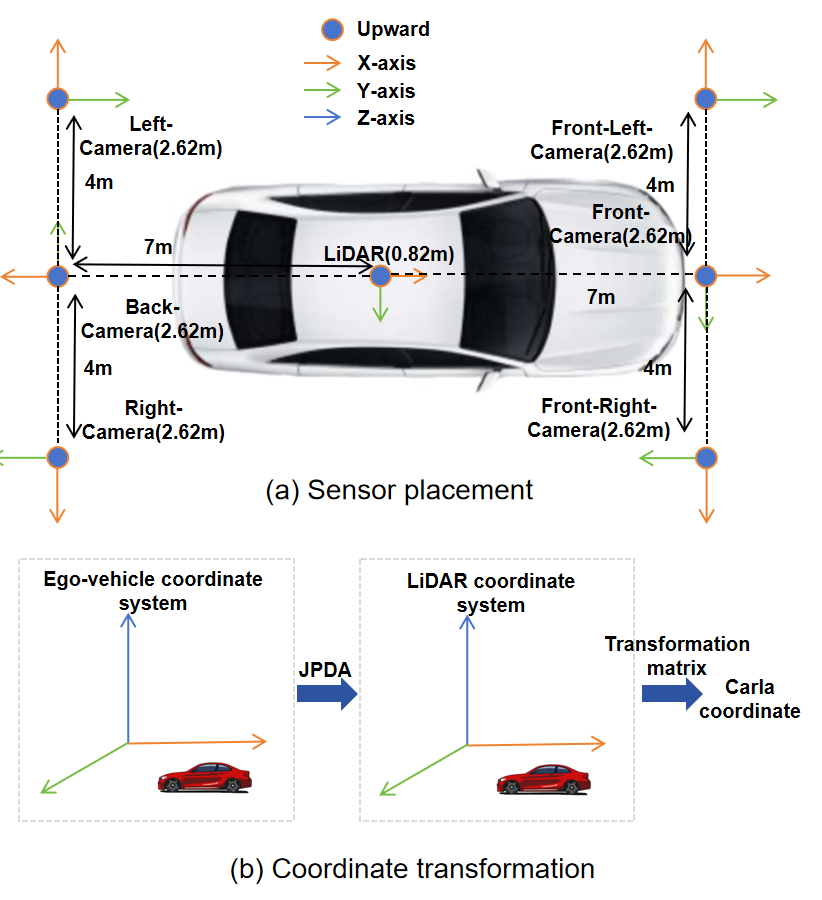
\includegraphics[width=\linewidth]{picture/picture3.png} 
	\caption{Trajectory restoration schematic} 
	\label{fig:3} 
\end{figure}

\subsection{Twin of Trajectory}

Through the previous steps, we have obtained the trajectories of all vehicles. 
Here, we will further optimize these trajectories using a trajectory smoothing algorithm, and then employ a PID controller to control the vehicles, ensuring they follow the optimized trajectories\cite{Alpher22d}. 
The PID controller consists of three main components: Proportional control (P), Integral control (I), and Derivative control (D). Each component serves a specific purpose, enabling the regulation of different aspects of the system.

$\bullet$ The proportional control component adjusts the control output directly based on the current error. 
The control output is proportional to the error, meaning that the larger the error, the stronger the control action. 
The formula is as follows:
\begin{align}
	u_{P}(t) & = K_{p} \cdot e(t)
\end{align}
Here, $K_{p}$ is the proportional gain, which determines the strength of the proportional control's response to the error.

Proportional control can quickly respond to errors and reduce their magnitude.
However, using only proportional control may not completely eliminate steady-state error, which is the small error that remains after the system has stabilized.

$\bullet$ The integral control component accumulates the sum of errors and adjusts the control output based on this accumulated value. 
The integral term takes into account historical errors and is capable of eliminating steady-state errors. 
The formula is as follows:
\begin{align}
	u_{I}(t) & = K_{i} \int_{0}^{t} e(\tau) d \tau
\end{align}
Here, $K_{i}$ is the integral gain, which determines the strength of the integral control's response to the accumulated error. 

By considering the accumulated error, integral control can eliminate steady-state errors, enabling the system to achieve the target value over the long term. 
However, excessively high integral gain may lead to system overshoot or oscillation.

$\bullet$ The derivative control component adjusts the control output based on the rate of change of the error. 
It predicts future error trends and takes preemptive measures. 
The formula is as follows:
\begin{align}
	u_{\mathit{D}}(t) & = K_{d} \cdot \frac{d e(t)}{d t}
\end{align}
Here, $K_{d}$ is the derivative gain, which determines the strength of the derivative control's response to the rate of change of the error.

Derivative control can suppress rapid changes in errors, reduce system overshoot and oscillation, and make the system response smoother. 
However, derivative control is sensitive to noise and can amplify high-frequency noise.


The tuning process of the PID controller is as follows:  
1. Calculate the error $e(t)$ between the target value (setpoint) and the current system output in real time.  
2. Compute the proportional action $K_{p} \cdot e(t)$ based on the current error, the integral action $K_{i} \int_{0}^{t} e(\tau) d \tau$ based on historical errors, and the derivative action $K_{d} \cdot \frac{d e(t)}{d t}$ based on the rate of change of the error.  
3. Sum the results of the proportional, integral, and derivative components to obtain the final control output $u(t)$, which is then applied to the system (for example, adjusting the vehicle's acceleration or direction). 
4. The system adjusts based on the control output $u(t)$, changing its state (for example, speed, position, etc.). 
The controller continues to monitor the system state, updates the error in real time, and repeats the above steps until the system stabilizes near the target value.


\subsection{Evaluation}

We employed two evaluation metrics.

\textbf{Multiple Object Tracking Accuracy.}
Single-camera, multi-object tracking performance is typically measured by the Multiple Object Tracking Accuracy (MOTA):
\begin{align}
	\mathit{MOTA} & = 1-\frac{F N+F P+M}{T}
\end{align}
Among them:
$FN$ (False Negatives) represents the number of missed detections, which means targets that truly exist but were not detected.
$FP$ (False Positives) represents the number of false detections, which means targets that were detected but do not actually exist.
$M$ (Mismatches) represents the number of identity mismatches, which means cases where the tracking ID of a target was incorrectly assigned during the tracking process.
$T$ (Total number of true detections) represents the total number of true detections, which means the number of targets correctly detected across all frames.

The value of MOTA ranges from 0 to 1, with higher values indicating better tracking performance. 
A MOTA of 1 means there are no missed detections, false detections, or identity mismatches, representing perfect tracking performance. 
A MOTA of 0 means the tracking performance is very poor, with all detections being incorrect.

\textbf{Multi Camera Tracking Accuracy.}
The multi-camera object tracking accuracy (MCTA) which condenses all aspects of system performance into one measure\cite{Alpher23b}:
\begin{align}
	\mathit{MCTA} & = \frac{2 P R}{P+R}\left(1-\frac{M^{w}}{T^{w}}\right)\left(1-\frac{M^{h}}{T^{h}}\right)
\end{align}
Among them:
$P$ represents the proportion of correct matches (correctly identifying and tracking targets) across all cameras.  
$R$ represents the recall rate, which is the proportion of all true targets that are correctly tracked.  
$M^{w}$ represents the number of weak matching errors, which is the number of times a target is incorrectly matched to another target during the tracking process.  
$T^{w}$ represents the total number of weak matching attempts, which is the total number of possible matching attempts.  
$M^{h}$ represents the number of strong matching errors, which is the number of times a target is incorrectly matched to another target during the tracking process, but here it may refer to a stricter standard for matching errors.  
$T^{h}$ represents the total number of strong matching attempts, which is the total number of possible matching attempts.

MCTA evaluates tracking accuracy by considering the proportion of correct matches and the recall rate, while also assessing tracking consistency by penalizing weak and strong matching errors. 
The higher the MCTA value, the better the performance of the multi-camera tracking system.


\section{Experiments}

We conducted the following experiments: 
(a) using PointPillars combined with YOLOv4 for vehicle detection, 
(b) performing multi-object tracking at each intersection in the simulation scene,
(c) vehicle re-identification between intersections using a ReID network, and 
(d) implementing trajectory digital twins in Carla.

\subsection{Preparation}

\begin{table*}[t]
	\centering
	\caption{MULTI-OBJECTIVE TRACKING EVALUATION}
	\label{tab:tracking_eval}
	\small
	\begin{tabular}{@{}l@{\hspace{1em}}c@{\hspace{0.5em}}*{10}{r}@{}}
		\toprule
		\textbf{Scene} & \textbf{Int.} & \textbf{Rcll} & \textbf{Prcn} & \textbf{FTR} & \textbf{FP} & \textbf{FN} & \textbf{IDS} & \textbf{MT} & \textbf{ML} & \textbf{MOTA} & \textbf{MOTP} \\
		\midrule
		\multirow{5}{*}{\shortstack[l]{Town01 \\ (16 int., flat roads, \\ sparsely popu- \\ lated buildings)}} 
		& 1 & 30.1025 & 59.9258 & 0.5106 & 216 & 750 & 18 & 0.0000 & 37.5000 & 8.2945 & 79.9222\\
		& 2 & 64.8065 & 61.5385 & 1.0297 & 450 & 391 & 21 & 55.5556 & 33.3333 & 22.4122 & 86.7746\\
		& 3 & 63.2135 & 45.4407 & 1.1887 & 359 & 174 & 15 & 0.0000 & 25.0000 & -15.8562 & 86.9053\\
		& 4 & 65.8206 & 96.7662 & 0.0369 & 13 & 202 & 20 & 40.0000 & 20.0000 & 60.2369 & 89.0919\\
		& 5 & 41.4035 & 90.0763 & 0.0580 & 13 & 167 & 10 & 50.0000 & 0.0000 & 33.3333 & 88.2471\\
		\midrule
		\multirow{5}{*}{\shortstack[l]{Town10 \\ (7 int., high-density, \\ including steep \\ slopes)}} 
		& 1 & 30.6653 & 59.7166 & 0.7960 & 398 & 1334 & 28 & 8.3333 & 50.0000 & 8.5239 & 84.6488\\
		& 2 & 56.4410 & 70.6095 & 1.1380 & 569 & 1055 & 29 & 13.3333 & 26.6667 & 31.7506 & 81.0920\\
		& 3 & 51.9805 & 75.6714 & 0.6160 & 308 & 885 & 17 & 14.2857 & 35.7143 & 34.3462 & 84.2826\\
		& 4 & 52.1930 & 86.1427 & 0.2680 & 134 & 763 & 50 & 27.2727 & 36.3636 & 40.6642 & 88.6035\\
		& 5 & 45.4243 & 62.2719 & 1.6540 & 827 & 1640 & 35 & 12.5000 & 37.5000 & 16.7388 & 86.0825\\
		\bottomrule
	\end{tabular}
\end{table*}

\textbf{Simulation Environment.}
We conducted simulation experiments in Carla, whose advantage lies in its provision of a highly realistic virtual environment capable of accurately simulating complex traffic scenarios and diverse driving conditions. 
Carla supports flexible sensor configurations, such as cameras and LiDAR, facilitating multimodal data acquisition and fusion experiments\cite{Alpher22e}. 
We conducted relevant experiments in the Town10 and Town01 scenes in Carla.
The complex urban structure and dense traffic flow of Town10 can simulate highly dynamic real traffic environments, while the simple layout and clear rules of Town1 make it easy to construct controlled experimental scenarios.
This scene diversity can effectively verify the generalization ability of the model under different traffic conditions and provide a reliable basis for actual road deployment.

\textbf{Data Collection.}
In CARLA's Town10 scenario, a single intersection location is selected, with a LiDAR placed at the center and six cameras arranged around it to achieve 360-degree omnidirectional perception coverage. 
This setup allows for the acquisition of rich point cloud data and image information, making it suitable for target recognition and tracking in complex traffic environments. 
By configuring the LiDAR with 64 channels, a detection range of 100 meters, 250,000 points per second, and a rotation frequency of 20 Hz, the radar can efficiently generate high-density and accurate point cloud data. 
Additionally, one camera is placed at the front and rear of the vehicle, and one camera is positioned on each of the four roads to the left and right. 
The cameras have a resolution of 1920x1080 pixels and a field of view of 90 degrees, ensuring the capture of wide-angle image data in high definition. 
The collected data includes point cloud data from the LiDAR and image data from the cameras. 
The radar data is saved as MAT files with timestamps, while the camera data is saved as images for each frame in six directions. 
The data structure follows the storage format of the Panda dataset, making the data more standardized for subsequent processing and fusion\cite{Alpher21c}. 
Each frame of data synchronously collects six-directional camera images and LiDAR data containing point clouds, timestamps, and the coordinates of the sensor relative to the ego-vehicle.

\subsection{Experimental Effect}

\textbf{Multi-Object Tracking.}
Table 2 presents the multi-object tracking performance metrics across different scenarios (Town01 and Town10) and intersections (Intersection 1-5). 
The data reveals significant variations in performance across different intersections. 
In Town01, Intersection 4 shows better performance in terms of Recall (65.8206) and Precision (96.7662), while Intersection 3 has a higher False Track Ratio (1.1887), indicating a greater proportion of incorrect tracking. 
In Town10, Intersection 4 also demonstrates relatively high Recall (52.1930) and Precision (86.1427), but Intersection 5 has significantly higher False Positives (827) and False Negatives (1640) compared to other intersections, suggesting a higher number of misidentified and missed targets.

Identity Switches (IDS) are notably higher in Intersection 4 of both Town01 and Town10, with values of 20 and 50 respectively, indicating more frequent target identity switches at these intersections. 
The Mostly Tracked (MT) and Mostly Lost (ML) metrics show that Intersection 2 in Town01 has a higher MT (55.5556), while Intersection 1 in Town10 has a higher ML (50), reflecting significant differences in tracking stability across these intersections.

Overall, the MOTA (Multiple Object Tracking Accuracy) and MOTP (Multiple Object Tracking Precision) metrics indicate that Intersection 4 in Town01 performs well with MOTA (60.2369) and MOTP (89.0919), whereas Intersection 5 in Town10 has a lower MOTA (16.7388), suggesting poorer overall tracking accuracy. 
These data highlight the performance variations of the multi-object tracking system across different scenarios and intersections, providing valuable insights for further optimization.

\textbf{Twin.}
The performance of the digital twin is primarily reflected by two sets of metrics: trajectory coincidence and control error (as shown in Tables 3 and 4). 
These two tables compare the performance evaluation metrics of the digital twin in two scenarios, Town01 and Town10. 
The trajectory overlap rate (TOR) in Town01 (50.21\%) is significantly higher than that in Town10 (10.89\%), indicating superior path-tracking capability, possibly due to a simpler environment or more stable control algorithms. 
In terms of mean position error (MPE), the two are close (Town01: 79.58m, Town10: 82.41m). 
However, the maximum position error (MaxPE: 105.89m) and final position error (FPE: 105.09m) in Town10 far exceed those in Town01 (MaxPE: 33.14m, FPE: 19.90m), revealing severe localization deviations in extreme cases, likely caused by complex environments or dynamic obstacles. 
For mean lateral error (MLE) and mean longitudinal error (MLOE), Town10 performs slightly better (MLE: 1.98 vs. 2.19, MLOE: 0.26 vs. 0.53), suggesting more precise lateral and longitudinal control, though overall stability is lacking. 
In terms of mean delay (MD), Town01 (1.20 seconds) outperforms Town10 (1.38 seconds), demonstrating higher task execution efficiency.


\begin{table}[t]
	\centering
	\caption{Table of the trajectory indicator}
	\label{tab:improved}
	\begin{tabular}{|c|c|c|c|c|c|}
		\hline
		Type & Scene & TOR(\%) & MPE(m) & MaxPE(m) & FPE(m) \\
		\hline
		\multirow{2}{*}{TRACK-DT} & Town01 & 50.2143 & 79.5798 & 33.1382 & 19.8970 \\
		\cline{2-6}
		& Town10 & 10.8957 & 82.4108 & 105.8893 & 105.0854 \\
		\hline
		\multirow{2}{*}{TRACK-GT} & Town01 & 18.4326 & 59.3773 & 79.6541 & 64.0980 \\
		\cline{2-6}
		& Town10 & 34.4533 & 52.5575 & 36.0566 & 31.4600 \\
		\hline
	\end{tabular}
\end{table}

\begin{table}[t]
	\centering
	\caption{Table of the error and delay indicators}
	\label{tab:improved}
	\begin{tabular}{|c|c|c|c|}
		\hline
		\multicolumn{1}{|c|}{Scene} & \multicolumn{1}{c|}{MLE} & \multicolumn{1}{c|}{MLOE} & \multicolumn{1}{c|}{MD(s)} \\
		\hline
		Town01 & 2.1889 & 0.5345 & 1.2015 \\
		\hline
		Town10 & 1.9835 & 0.2614 & 1.3780 \\
		\hline
	\end{tabular}
\end{table}

\subsection{Details Explanation}

We conducted ablation studies on LiDAR detection and multi-intersection multi-object tracking in object detection to ensure that our experiments achieved the desired results.

\textbf{LiDAR Detection.}
During LiDAR detection, we established a threshold for the detection results: targets exceeding the threshold were identified as vehicles, while those below the threshold were excluded as other objects. 
We conducted three experiments with thresholds set at 0.4, 0.5, and 0.6, respectively. 
The best results were achieved with a threshold of 0.5, which not only maximized the identification of vehicles but also effectively filtered out other clutter. 
At a threshold of 0.4, some non-vehicle objects, such as trees and buildings, were mistakenly identified as vehicles, and in some cases, cargo loaded on vehicles was even misclassified as a separate vehicle, significantly reducing recognition accuracy. 
Conversely, a threshold of 0.6 led to the missed detection of some vehicles, such as smaller cars, which were occasionally misclassified as boxes and overlooked.

\textbf{Multi-Intersection and Multi-Object Tracking.}
In the multi-intersection multi-target tracking experiment, the most critical task is the re-identification of vehicles across different intersections. 
Therefore, we also set a threshold for the re-identification results: if the similarity score exceeds the threshold, the targets are considered the same vehicle; otherwise, they are deemed different vehicles. 
During the experiment, we adjusted the threshold multiple times, testing values of 0.6, 0.65, 0.7, 0.8, and 0.9. 
Ultimately, we found that a threshold of 0.65 yielded the best re-identification performance. 
When the threshold was set higher than 0.65, some vehicles failed to match across intersections, and the higher the threshold, the more vehicles were unable to be successfully matched. 
Conversely, when the threshold was set lower than 0.65, it led to incorrect matches for some vehicles.

\subsection{Parameter Optimization}

\textbf{Background and Objectives.}
In order to further improve the performance of the tracker highly depends with the hyperparameter setting. 
Traditional manual parameter tuning is inefficient and difficult to find the global optimal solution. 
For this reason, we adopt a Bayesian Optimization (BOM) approach to automatically optimize the following key parameters through an intelligent search strategy:

$\bullet$ DetectionProbability: control the reliability of sensor detection.

$\bullet$ ClutterDensity: sensitivity to filtering false detections.

$\bullet$ NewTargetDensity: threshold for target initialization.

$\bullet$ Confirmation/DeletionThreshold: trajectory lifecycle management.

$\bullet$ DeathRate: robustness to handling targets leaving the scene.

Optimization Goal: Maximize Tracking Accuracy (MOTA) while reducing ID Switches and Trajectory Fragmentation.

\textbf{Optimization Processes.}
Bayesian optimization is a hyper-parametric optimization method based on probabilistic models, which solves the global optimization problem of black-box functions by the strategy of “finding the best parameter with the least number of attempts”.
The process is as follows:
1.Maximizing tracking performance by fitting existing data with a Gaussian process and constructing an objective function model in a 6-dimensional parameter space; 
2.A small number of random parameter combinations are selected to calculate the value of the acquisition function, and the next parameter to be tested is selected (e.g., the point with the largest EI); 
3.Run the experiment to get the MOTA corresponding to the new parameters, add to the dataset, and repeat until the maximum number of iterations is reached or convergence is achieved.
The improvement results after optimization compared with before optimization are shown in Fig. \ref{fig:4}.   
\begin{figure}[t]
	\centering
	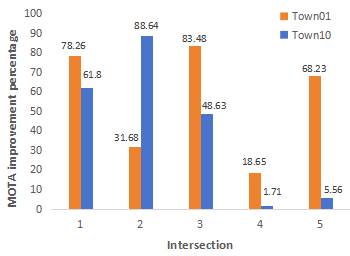
\includegraphics[width=\linewidth]{picture/picture4.png} 
	\caption{Trajectory restoration schematic} 
	\label{fig:4} 
\end{figure}

\subsection{Limitations and Future Directions}

\textbf{Problems Encountered in The Experiment.}
During our experiments, we encountered the following issues:  
1.When matching trajectories across multiple intersections, images of vehicles corresponding to each trajectory are needed to extract re-identification appearance features. 
Acquiring these images is difficult, and the methods used can affect accuracy.  
2.When matching trajectories, it is necessary to associate trajectories from all intersections. 
However, due to ID switching, the trajectory of the same vehicle at a single intersection may be fragmented, making integration complex. 
If only one trajectory is selected as the current intersection's trajectory for a vehicle, issues arise when the same vehicle returns to the intersection.

\textbf{Shortcomings of Current Research.}
Although our experiments have achieved some success, there are still some limitations. 
For example, the detection accuracy of PointPillars is not high, resulting in suboptimal tracking performance. 
Additionally, false detections may occur when acquiring images of vehicles corresponding to current trajectories, potentially leading to trajectory matching errors.

\textbf{Vision of The Future.}
Our experiments were conducted under offline conditions, meaning they lacked real-time capabilities. 
In future work, we aim to transition these experiments to an online framework to achieve high real-time performance, thereby enhancing their experimental value.


\section{Conclusion}

Through a series of experiments, we have demonstrated the application value of digital twins in intelligent transportation. 
Digital twin technology can not only accurately replicate real-world traffic scenarios but also effectively predict future traffic conditions. 
Multi-target tracking and the inference of unknown trajectories serve as strong evidence of this capability. 
This holds significant value for the development of future cities.

We hope that new large-scale datasets will be introduced in the future to further enhance the effectiveness of digital twins.


\bibliographystyle{IEEEtran}
\bibliography{reference}

\end{document}


